%
% System arkitektur
%
\chapter{System Arkitektur}

\begin{figure}[htbp] \centering
\section{Domænemodel}
{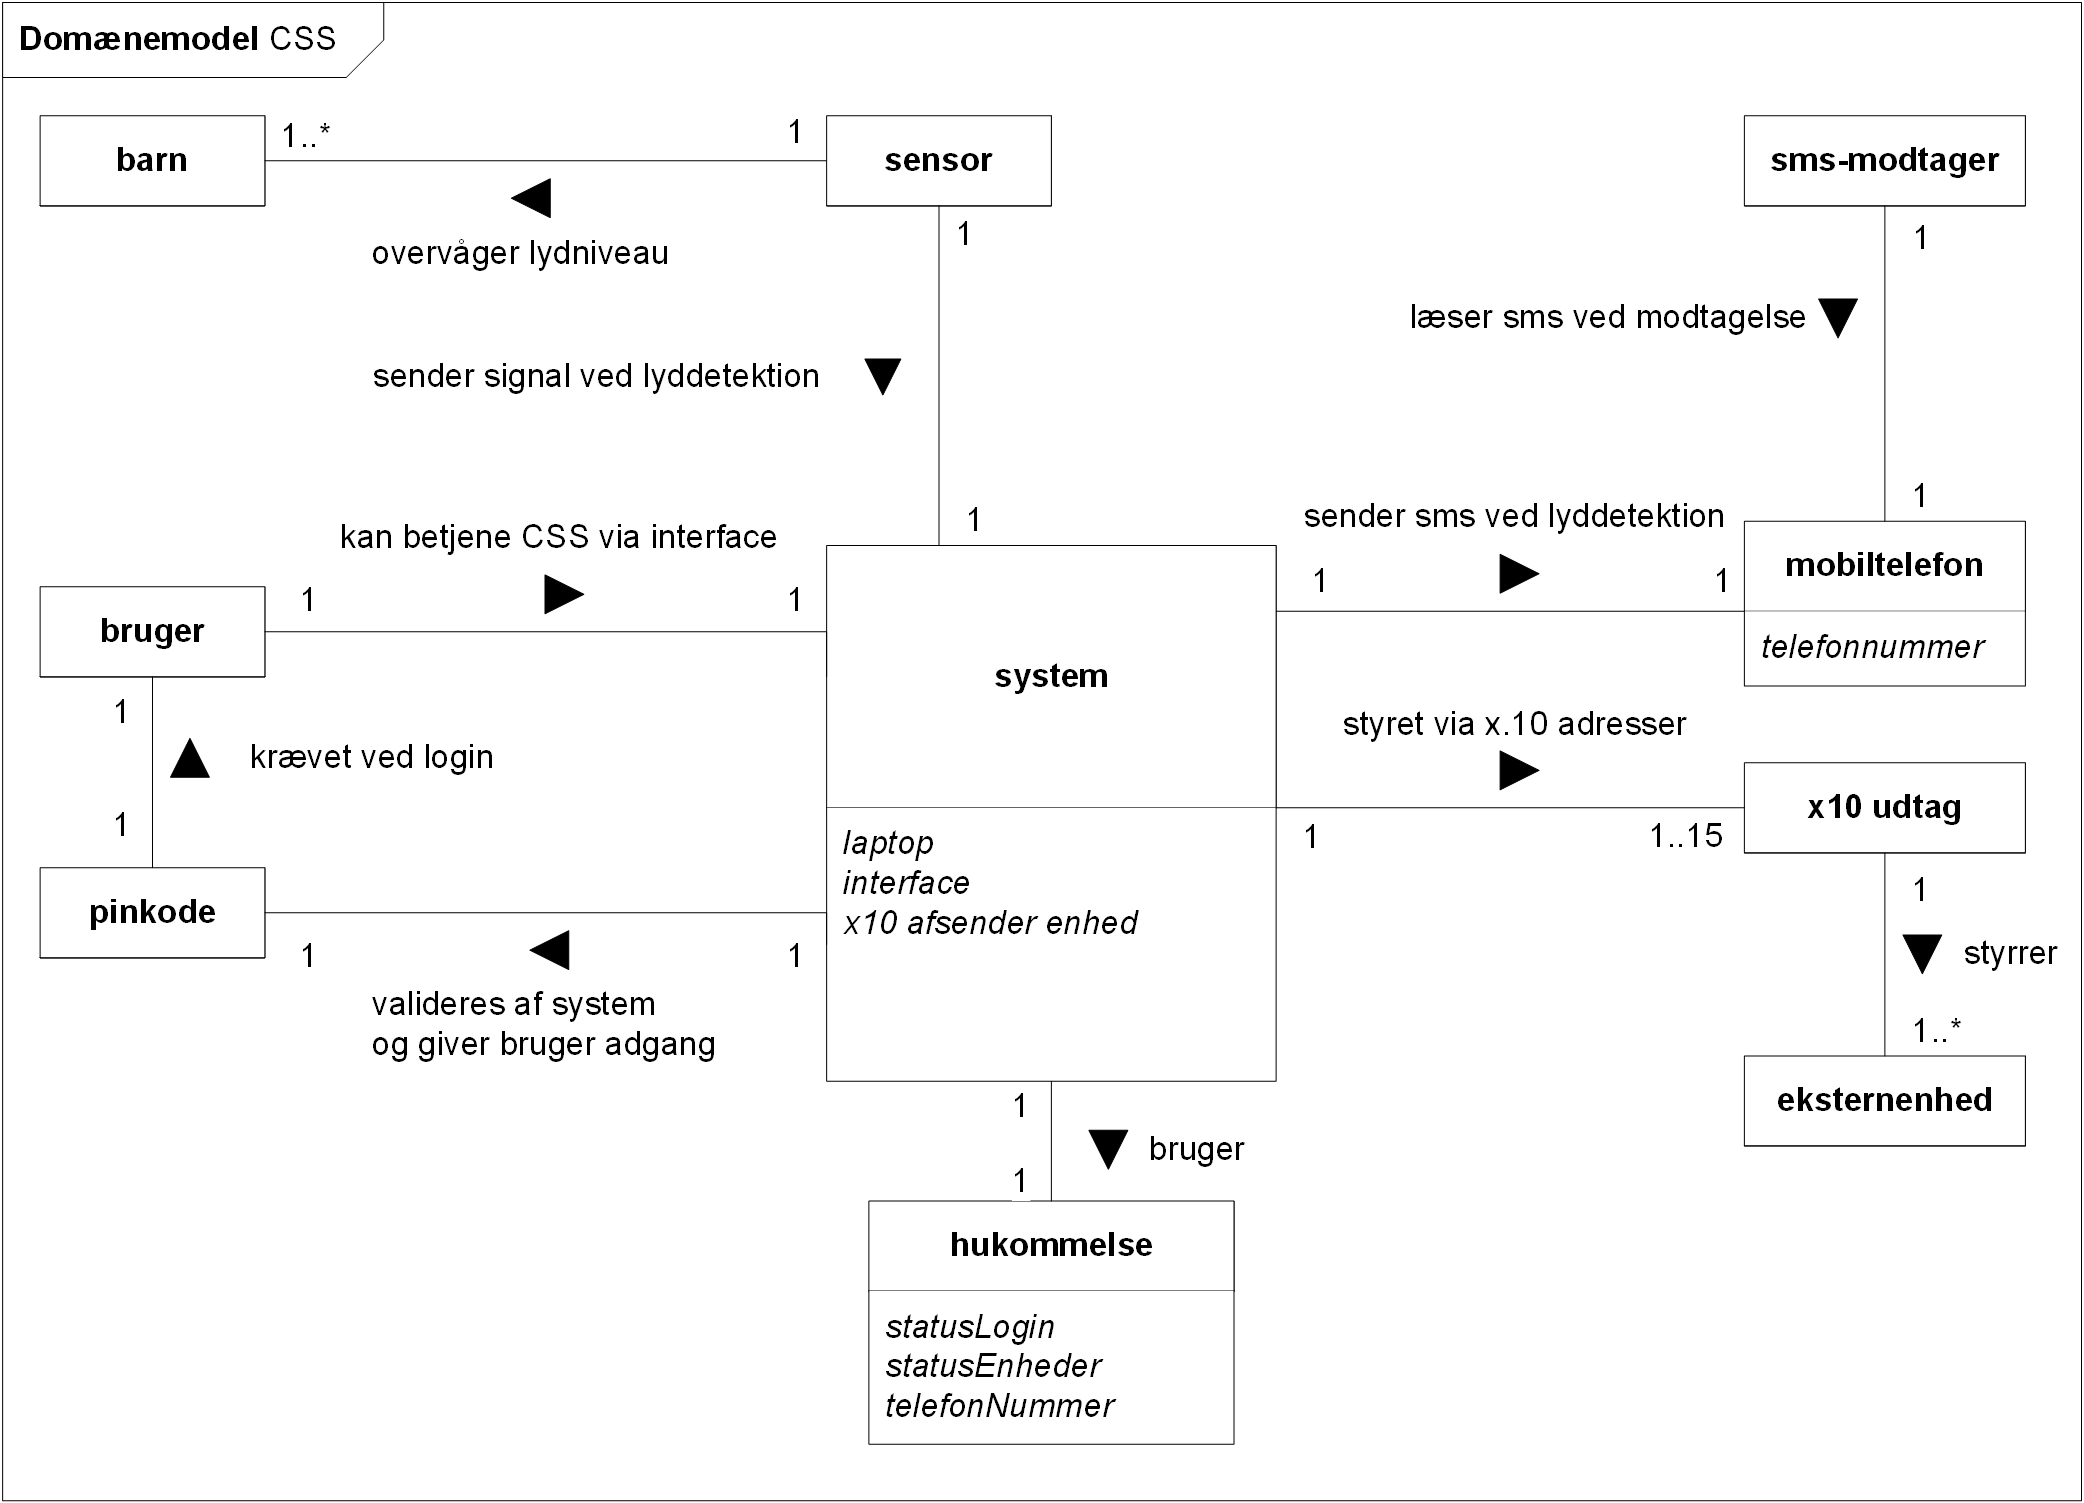
\includegraphics[width=\textwidth]{billeder/diagrammer/Domain_Model}}
\caption{Domænemodel}
\label{lab:domainmodel}
\end{figure}
Domænemodel er udarbejdet i samarbejde med kunden. Denne har til opgave at give et struktureret billede af systemets funktionalitet og sammenhæng. Domænemodellen gør ikke brug af fagudtryk, men pile og kortfattede samt præcise sætninger anvendes for at beskrive sammenhængen mellem blokkene. Dette er med til at opnå en højere forståelse, af systemet som helhed, for kunden.

\newpage
%% Hardware
\section{Hardware}

\subsection{Hardware beskrivelse}
\begin{figure}[!htbp] \centering
\subsection{BDD Hardware}
{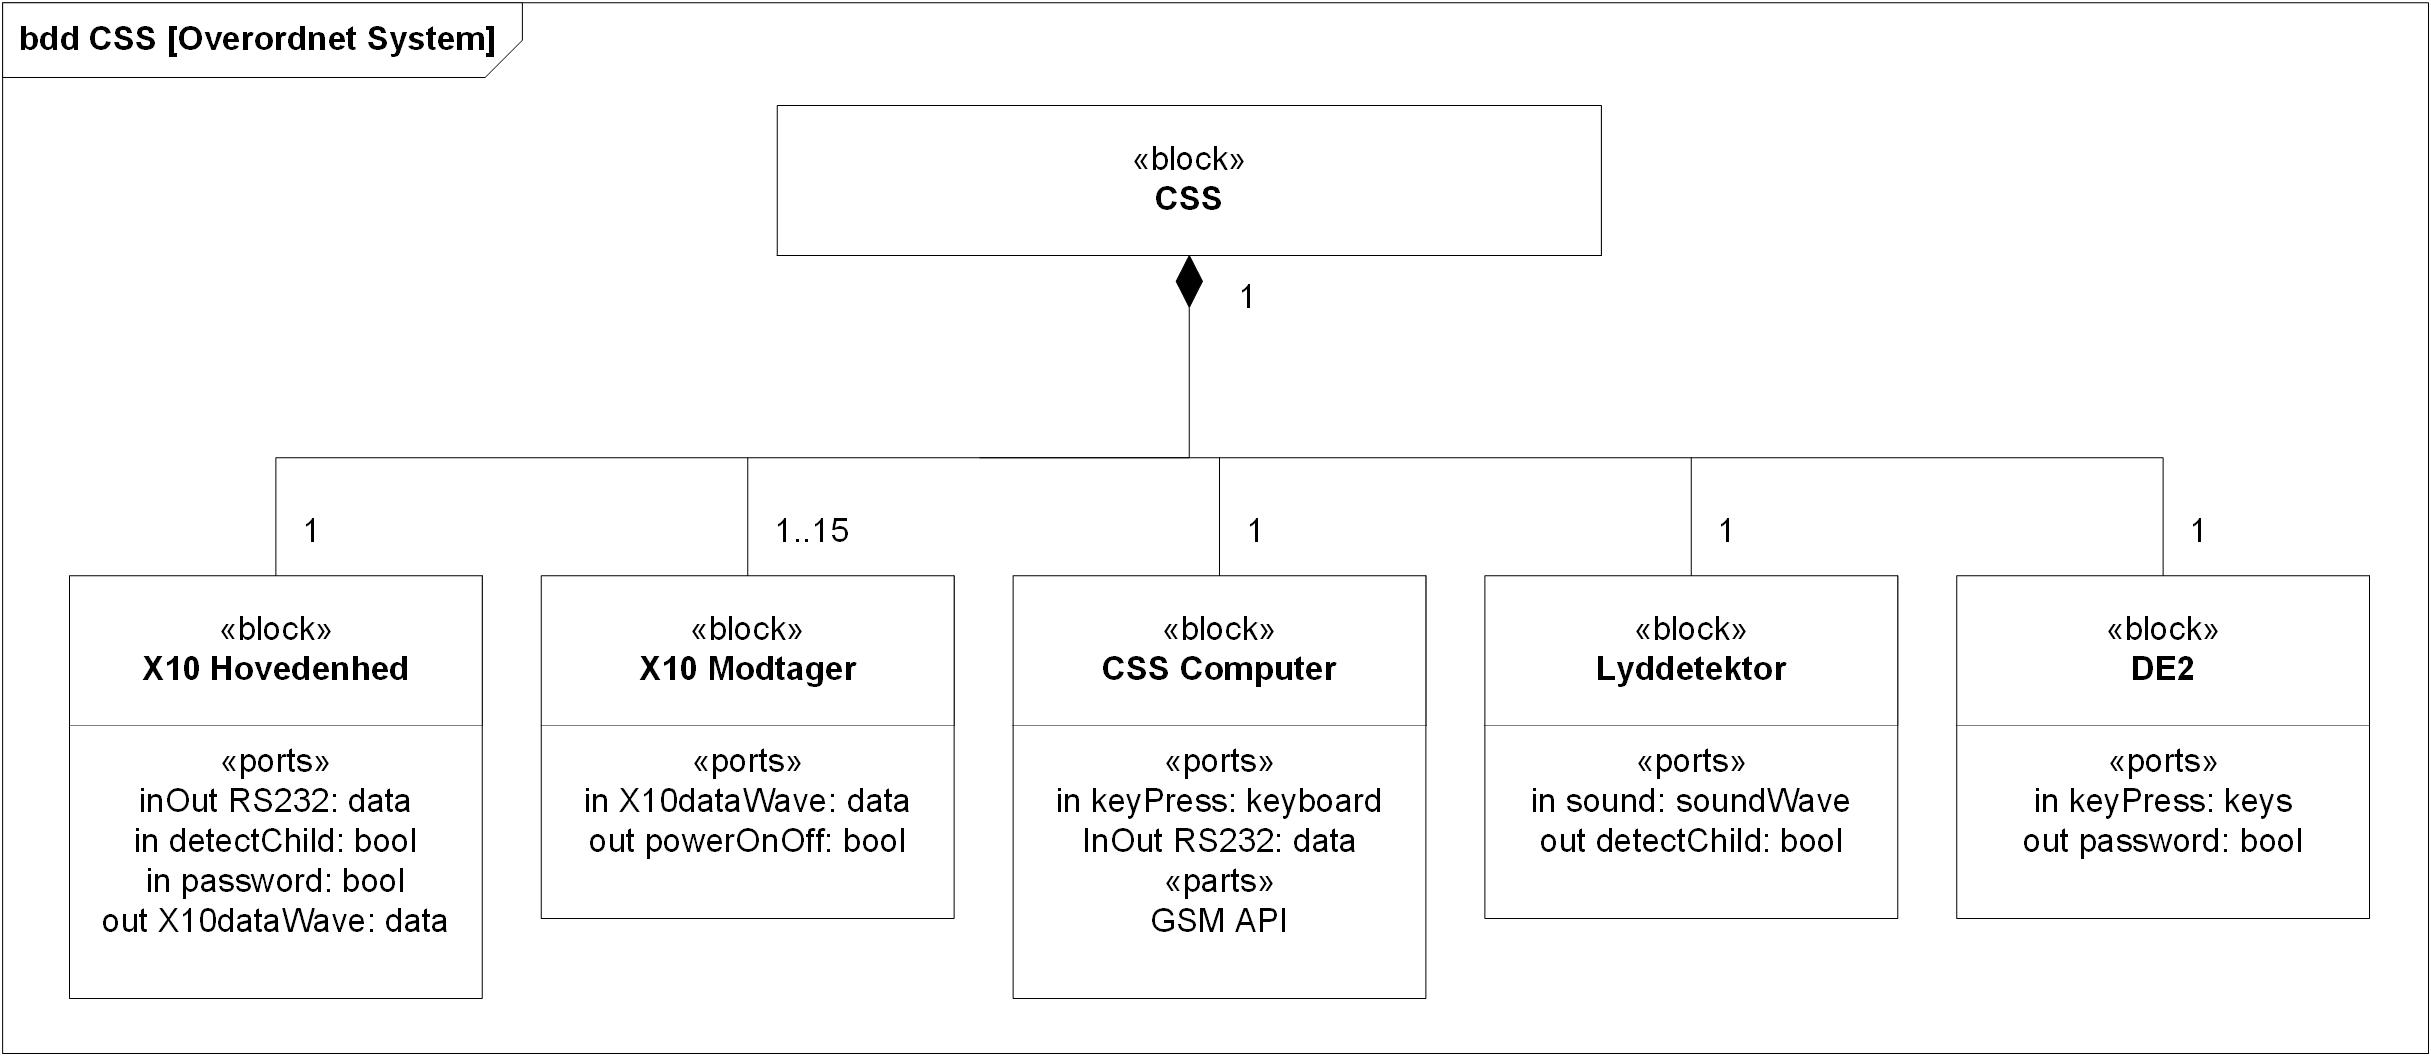
\includegraphics[width=0.9\textwidth]{billeder/diagrammer/BDD_Hardware}}
\caption{BDD Hardware}
\label{lab:bddhardware}
\raggedright
\end{figure}
BDD diagrammet giver et overblik over hvad det samlede system består af. Vi ser en port beskrivelse som viser hvilke signaler hver blok består af.

\begin{figure}[!htbp] \centering
\subsection{BDD Hovedenhed}
{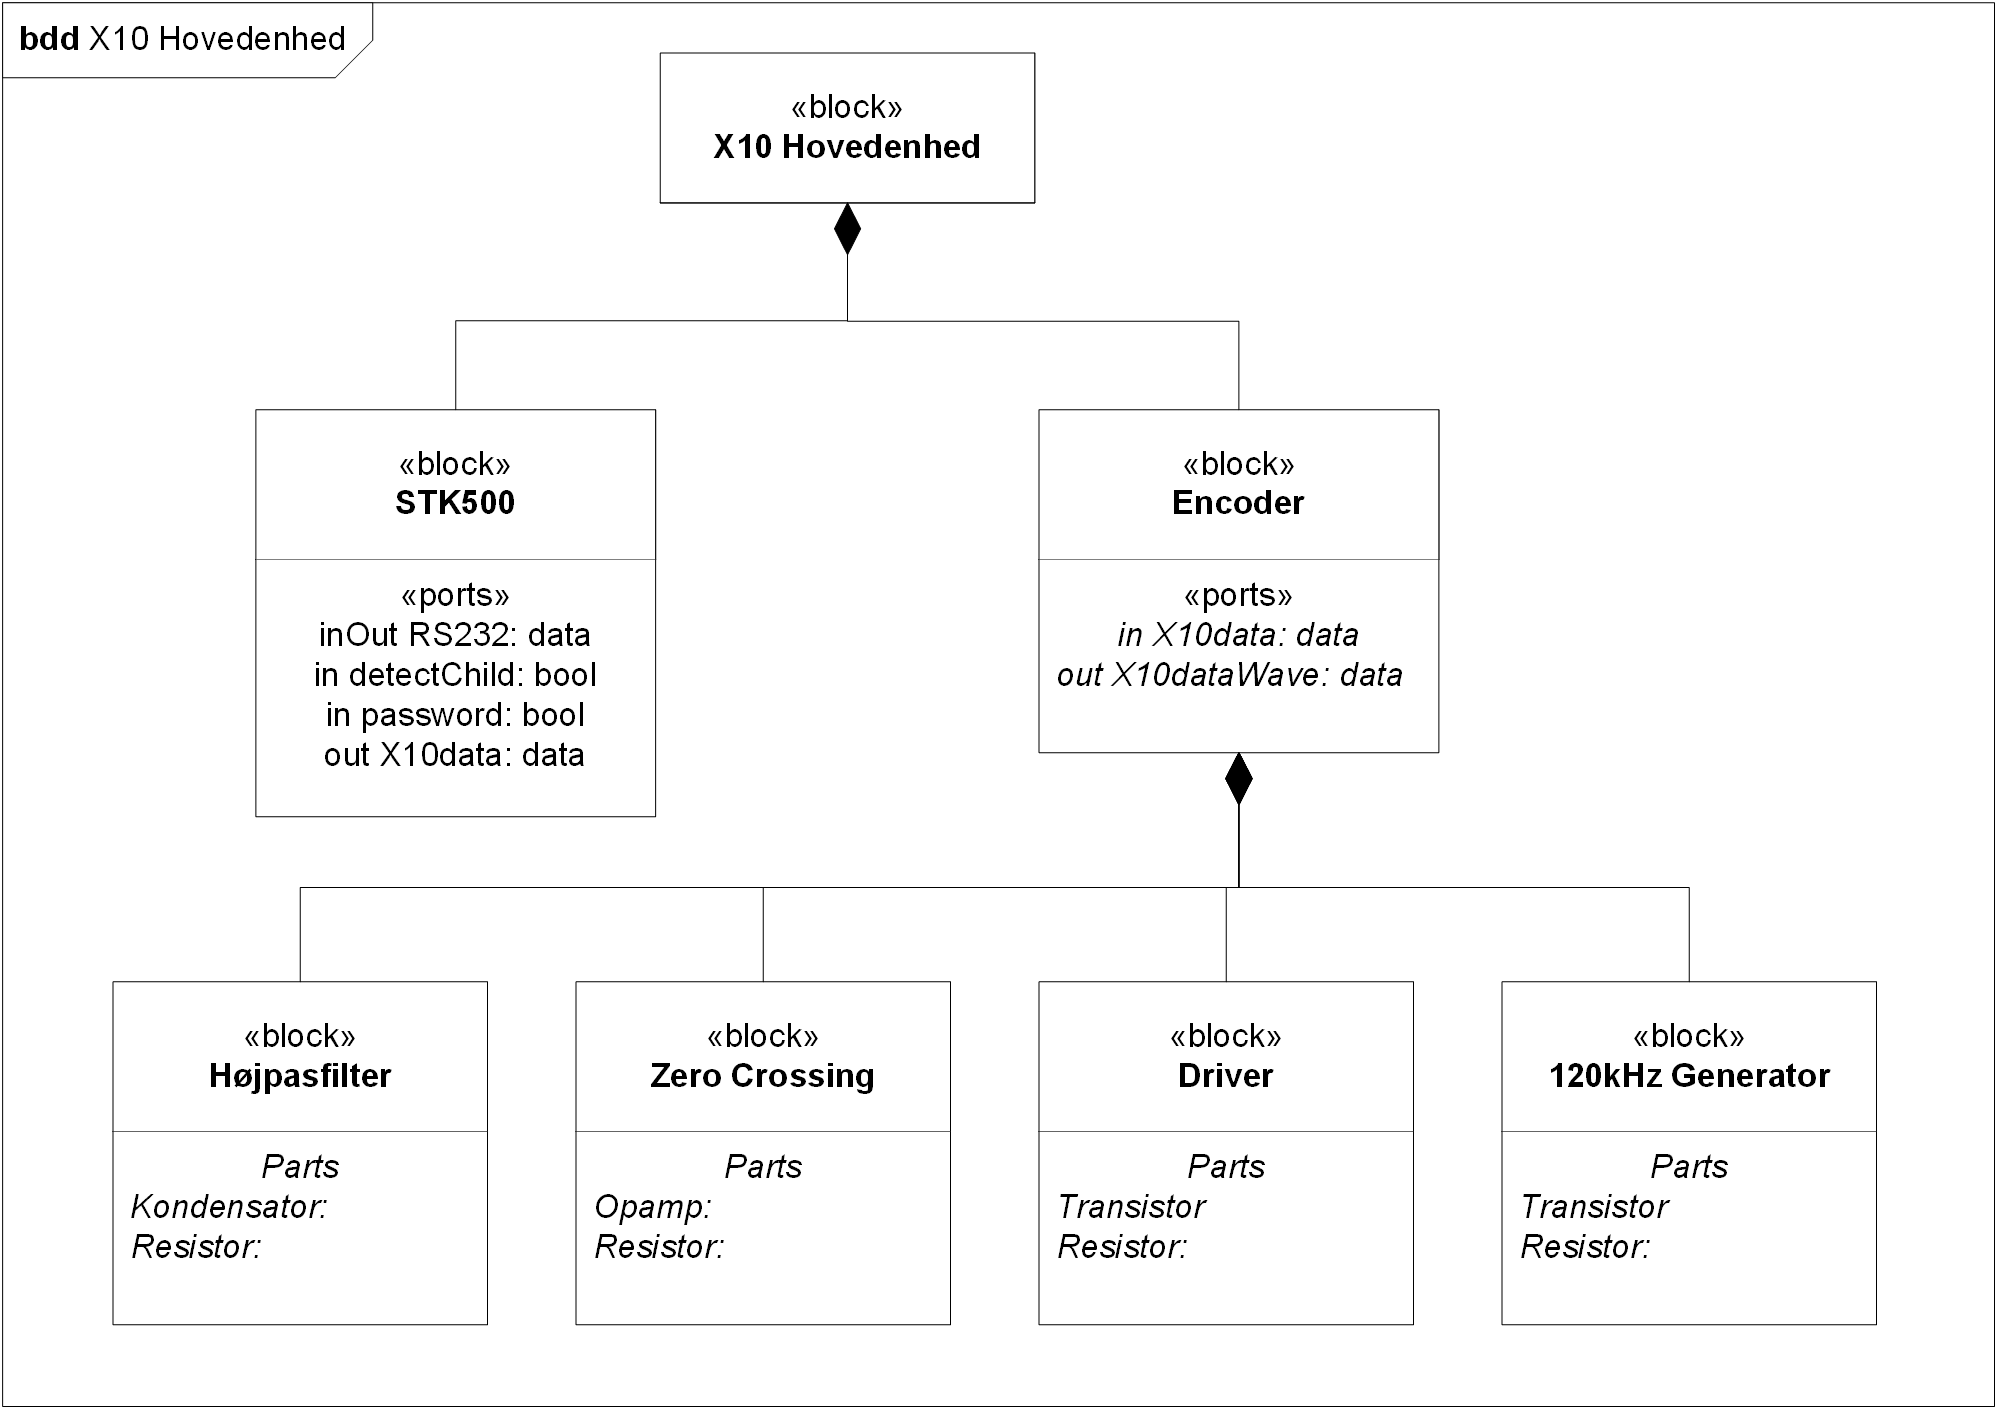
\includegraphics[width=0.9\textwidth]{billeder/diagrammer/BDD_Hovedenhed}}
\caption{BDD Hovedenhed}
\label{lab:bddhovedenhed}
\raggedright
\end{figure}
BDD diagrammet giver et overblik over hvad CSS hovedenheden består af. Vi ser en portbeskrivelse for STK kittet og encoder samt et overblik over hvilke komponenter encoderen består af. 

\begin{figure}[!htbp] \centering
\subsection{BDD Modtager}
{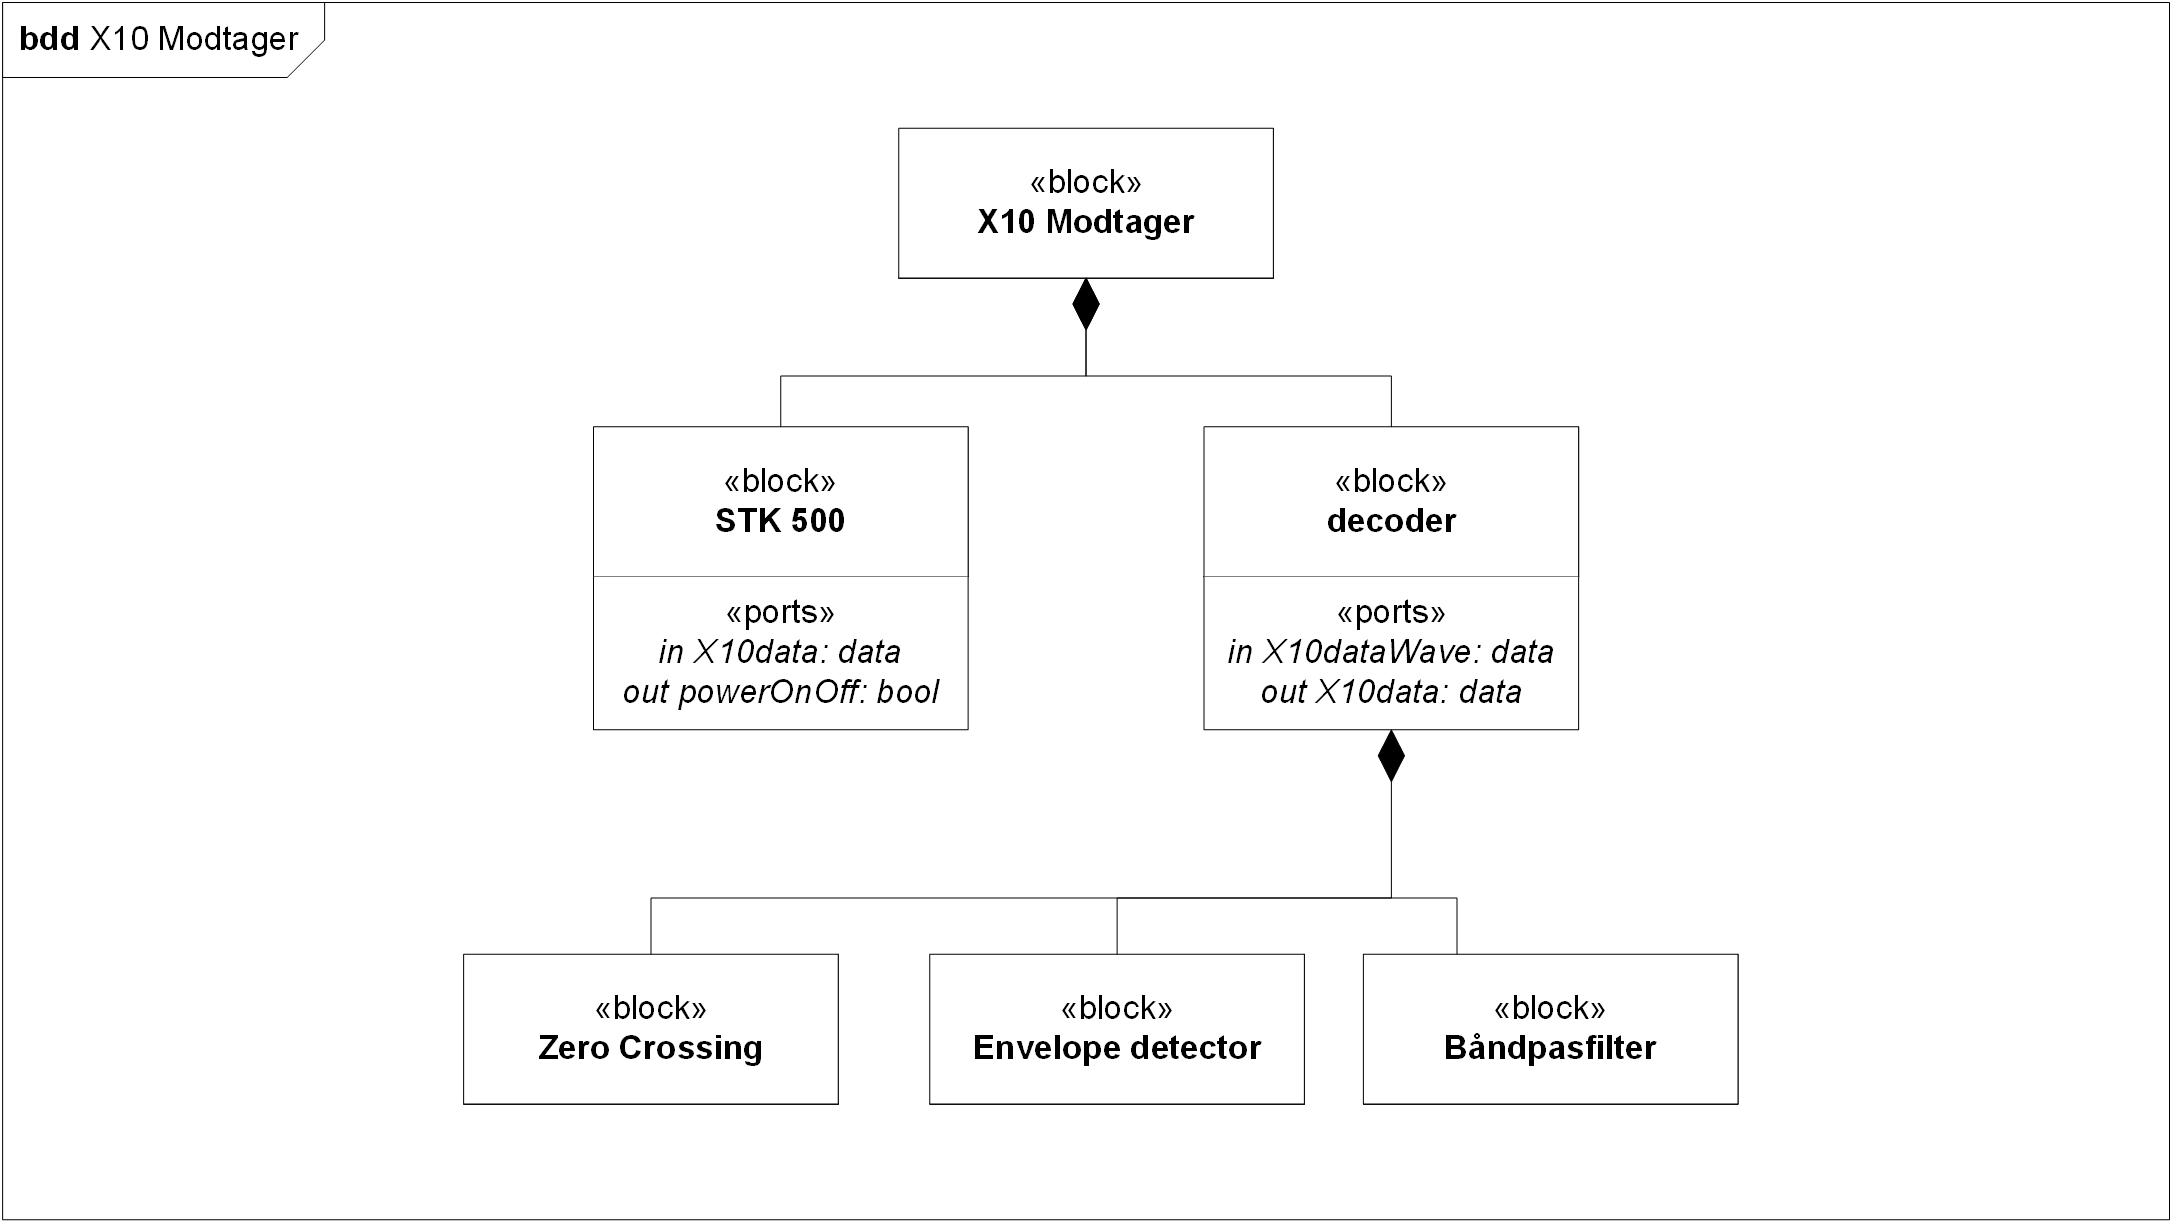
\includegraphics[width=0.9\textwidth]{billeder/diagrammer/BDD_Modtager}}
\caption{BDD Modtager}
\label{lab:bddmodtager}
\raggedright
\end{figure}
BDD diagrammet giver et overblik over hvad X10 modtageren består af. Vi ser en portbeskrivelse for STK kittet og decoderen samt et overblik over hvilke komponenter decoderen består af.

\begin{figure}[!htbp] \centering
\subsection{IBD Hardware}
{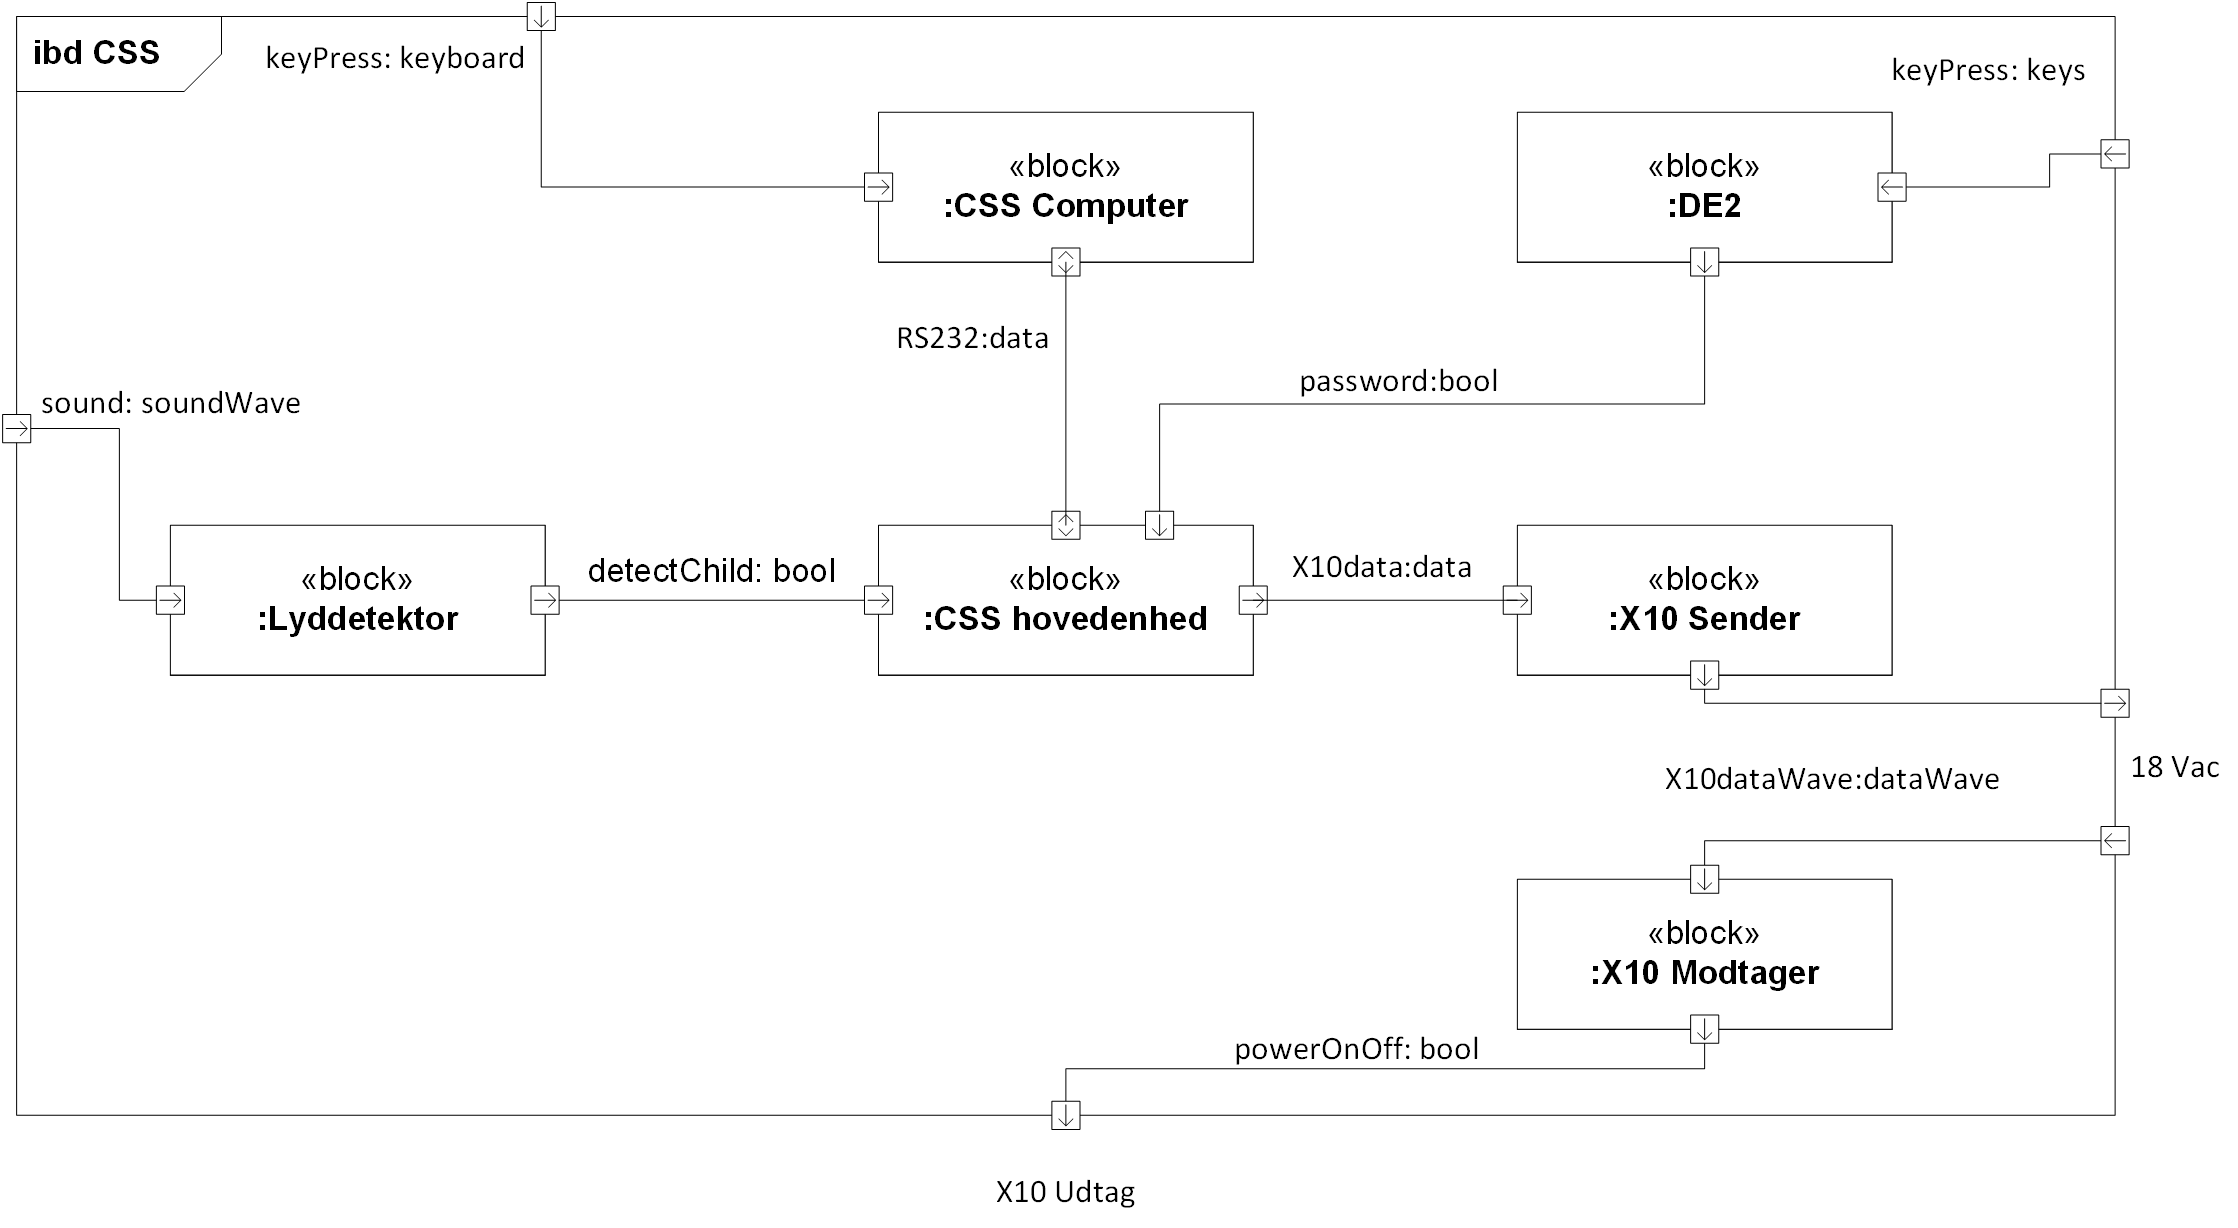
\includegraphics[width=0.9\textwidth]{billeder/diagrammer/IBD_Hardware}}
\caption{IBD Hardware}
\label{lab:ibdhardware}
\raggedright
\end{figure}
IBD diagrammet giver et internt overblik over hvordan hele vores system er forbundet. Vi ser hvilke type signaler der bliver sendt imellem vores forskellige blokke.

\begin{figure}[!htbp] \centering
\subsection{IBD Hovedenhed og Modtager}
{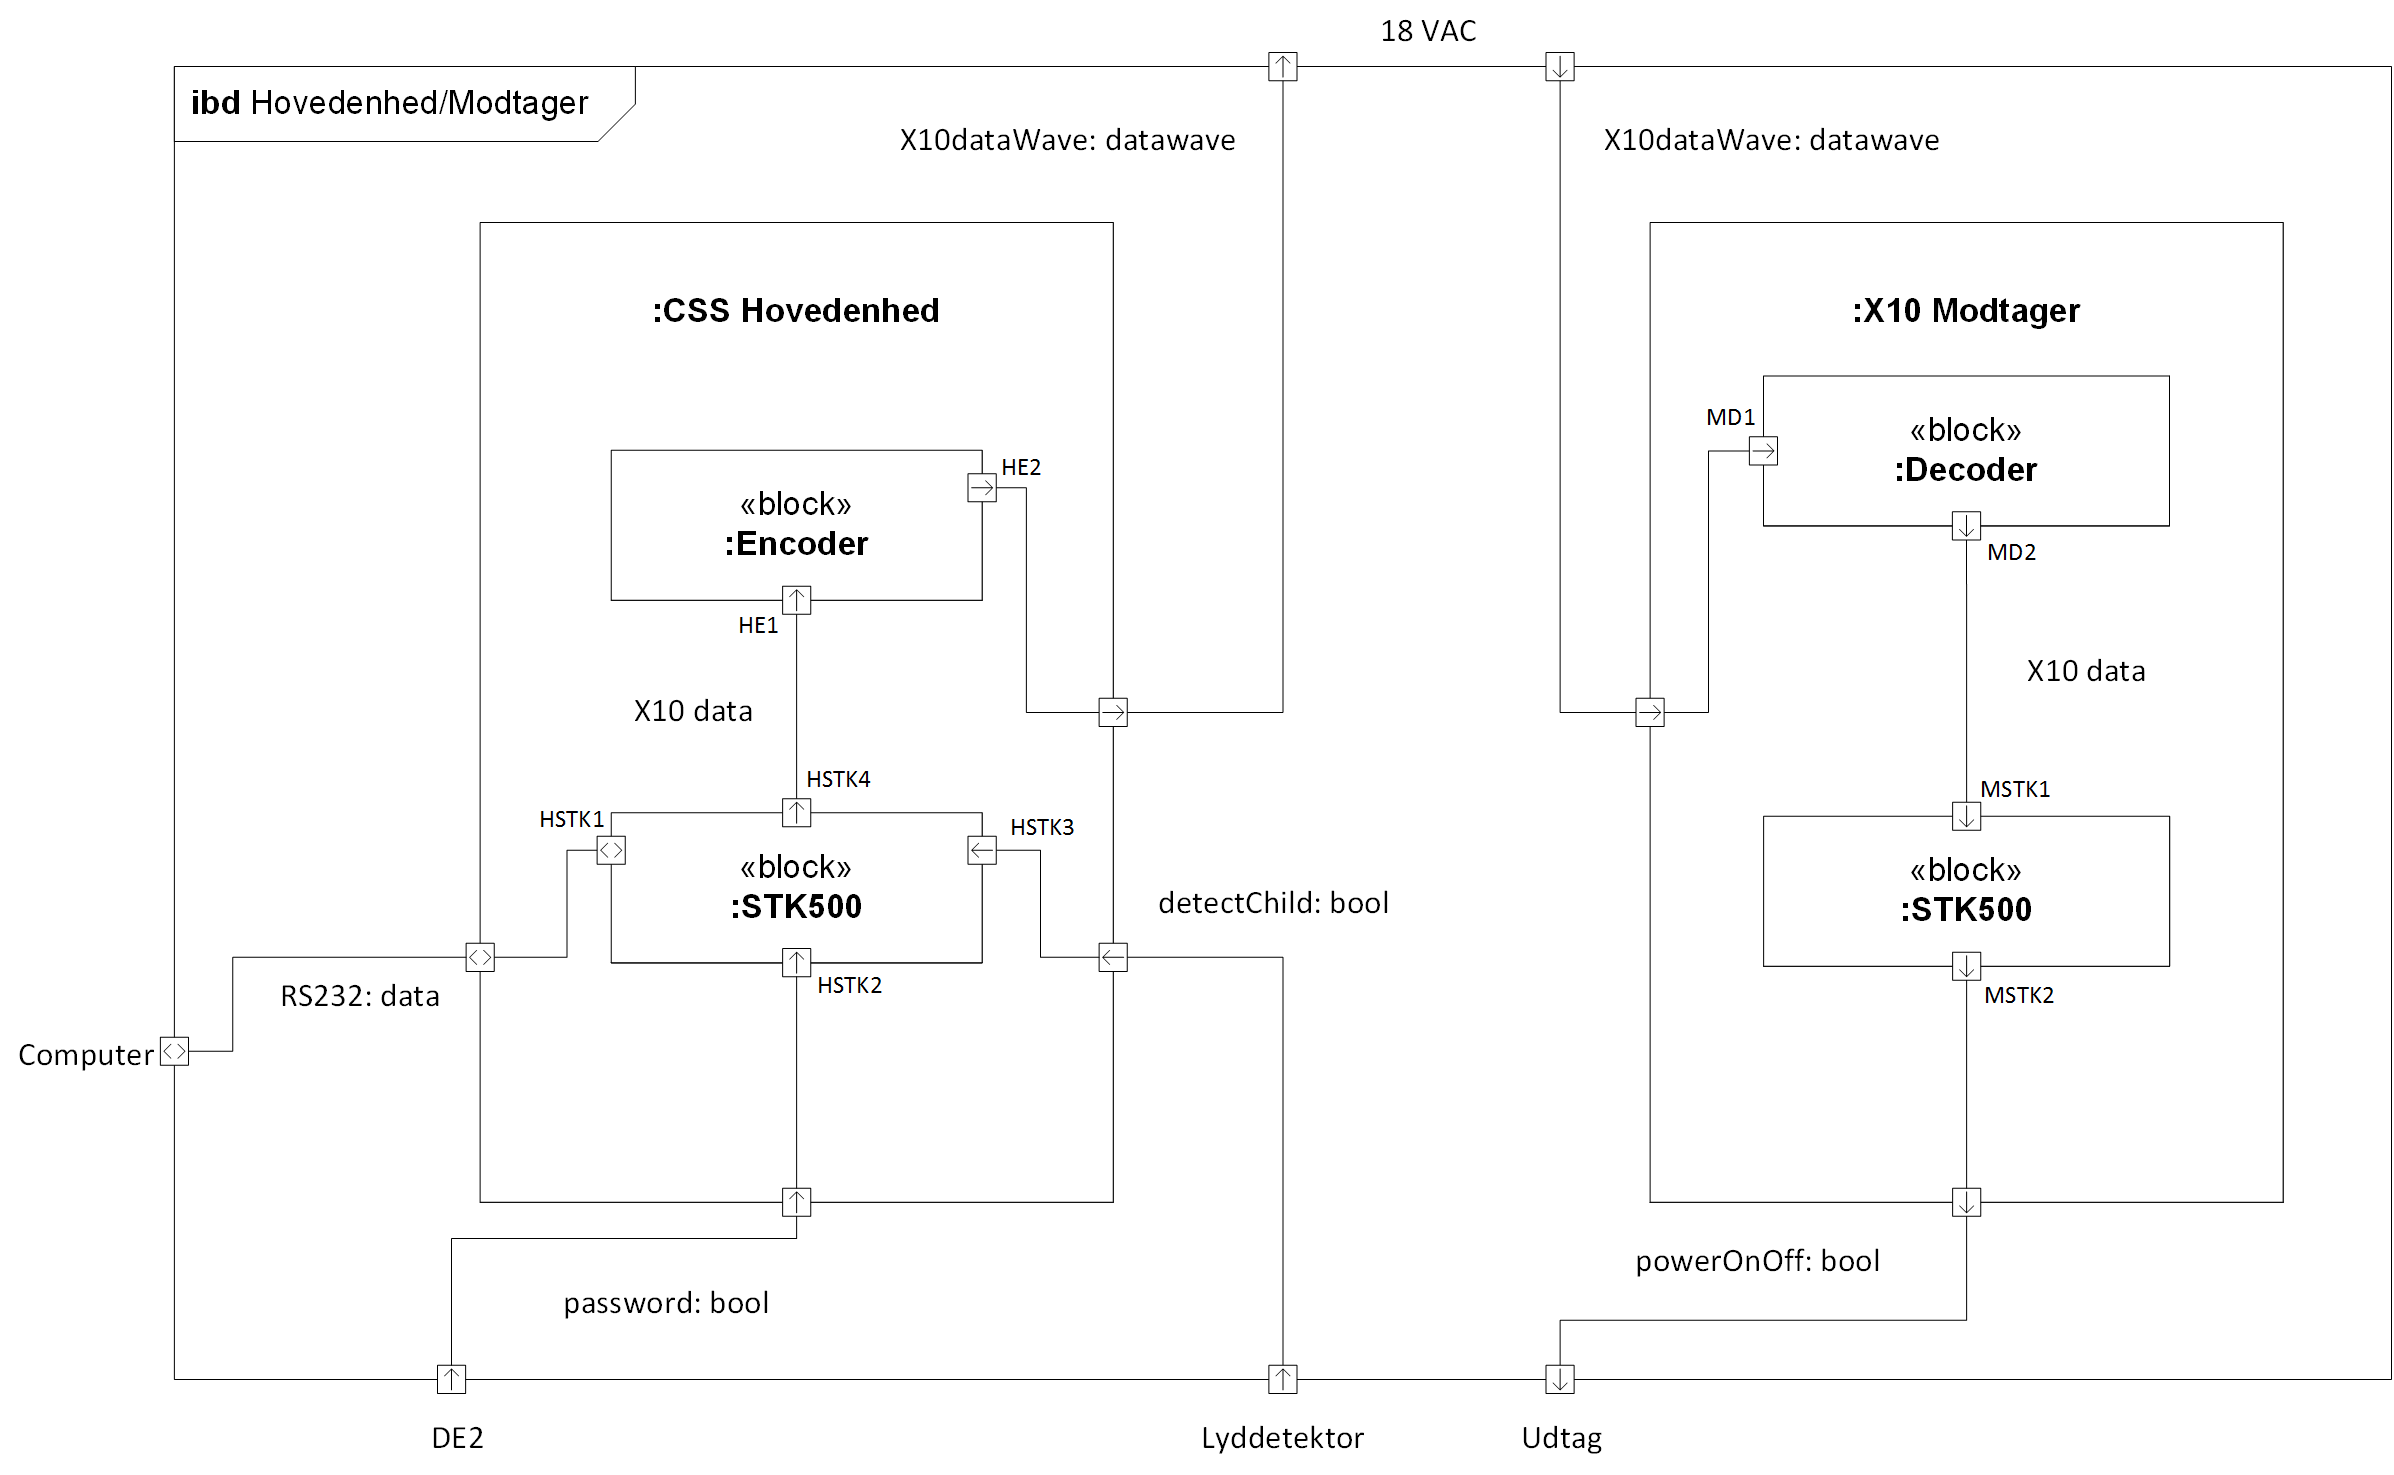
\includegraphics[width=0.9\textwidth]{billeder/diagrammer/IBD_Hovedenhed_Modtager}}
\caption{IBD Hovedenhed og Modtager}
\label{lab:ibdhovedenhedmodtager}
\raggedright
\end{figure}
IBD diagrammet giver et internt overblik over hvordan vores X10 hovedenhed og X10 modtager er forbundet. Vi ser hvilke type signaler der bliver sendt imellem vores forskellige blokke.


\clearpage
\newpage

\begin{table}[htbp] %% Blok og Signal Tabel
\subsection{Grænseflade}
For at opnå forståelse for signaler mellem blokkene laves en grænseflade der beskriver de enkelte blokkes porte og hvilke signaler der løber mellem disse.

\subsubsection{Blok beskrivelse}
Til at beskrive blokkene nærmere er anvendt tabeller som ses herunder. Her er hvert signal i en respektiv blok kommenteret og blokkens funktion er kort beskrevet. 

\caption{Tabel med beskrivelse af respektive blokke}
\begin{small}
\begin{tabular}{|p{3,3cm}|p{3,3cm}|p{3,3cm}|p{3,3cm}|}
\hline
\textbf{Bloknavn} & \textbf{Funktion} & \textbf{Signaler} & \textbf{Kommentar} \\ \hline

Encoder & modtage kommando og encode til 120 kHz bursts & 120 kHz & Data ud \\ \cline{3-4}	
& & X10 data & X10 data kommando ind \\ \hline

STK500 Hovedenhed & Genererer burst og detekterer på zero-crossing & RS232 & Laptop forbindelse \\ \cline{3-4}
& & X10 data & X10 data kommando linje \\ \cline{3-4}
& & Bool & lyd detektion \\ \cline{3-4}
& & Bool & Password accept \\ \hline

Decoder & Modtager 120 kHz og decoder til X10 data & 120 kHz & 120 kHz ind \\ \cline{3-4}
& & X10 data & Kommando linje \\ \cline{3-4}
& & 120 kHz & 120 kHz data ind \\ \hline

STK 500 Decoder & Modtager burst og detekterer på zero-crossing & X10 data & X10 data ind \\ \cline{3-4}
&& Bool & Power I/O ekstern enhed \\ \hline 
\end{tabular}
\end{small}
\label{table:Bloktabel}
\end{table}

\begin{table}[htbp]
\subsubsection{Signal beskrivelse}
For at fuldende beskrivelsen af grænsefladen er der lavet en signaltabel som kan ses herunder. Hvert signal er beskrevet og tilknyttet en kort kommentar. Området et signal er defineret under er også beskrevet. Blok og terminal indgår også. 
\caption{Tabel over signaler med terminaler}
\begin{small}
\begin{tabular}{|p{2cm}|p{2cm}|p{2cm}|p{2cm}|p{2cm}|p{2,2cm}|}
\hline
\textbf{Signal-navn} & \textbf{Funktion} & \textbf{Område} & \textbf{Port 1} & \textbf{Port 2} & \textbf{Kommentar} \\ \hline

120 kHz & sende kommando på 18V nettet & & Encoder, HE2 & Decoder, DM1 & \\ \hline

X10 data & kommando & & STK500, HSTK4 & Encoder, HE1 & \\ \cline{4-5}
&&& Decoder, MD2 & STK500, MSTK1 &\\ \hline

bool & digital signal & 5V/0V & DE2, N/A & STK500, HSTK2 & \\ \cline{4-5}
&&& Lyddetektor, N/A & STK500, HSTK3 & \\ \cline{4-5}
&&& STK500, MSTK2 & Udtag, N/A & \\ \hline
\end{tabular}
\end{small}
\label{table:Signaltabel}
\end{table}




\clearpage
%% Software
\section{Software}

%%% Applikationsmodel for PC
\subsection{Applikations model for PC}
\input{filer/UML/applicationsmodel_pc}
\clearpage

%%%% Klasse beskrivelser
\subsection{Klassebeskrivelse for PC}
Her følger klassebeskrivelser for alle klasser til PC. \\

{\centering
\textbf{Hukommelse klasse}\par
}

void saveLogin(bool); \\
\textbf{Parametre:} ingen \\
\textbf{Returværdi:} ingen \\
\textbf{Beskrivelse:} gemmer login status og bevare denne i 10 minutter \\

void saveStatus(bool, int adresse); \\
\textbf{Parametre:} bool til bestemmelse af om status er aktiv eller deaktiv. Int adresse til bestemmelse af status på adressen \\
\textbf{Returværdi:} ingen \\
\textbf{Beskrivelse:} gemmer status på enheden på pågældende adresse \\

void getEnheder); \\
\textbf{Parametre:} ingen \\
\textbf{Returværdi:} ingen \\
\textbf{Beskrivelse:} gemmer login status og bevare denne i 10 minutter \\

int getNumber(); \\
\textbf{Parametre:} ingen \\
\textbf{Returværdi:} gemte telefonnummer \\
\textbf{Beskrivelse:} returnere det gemte telefonnummer \\

void saveNumber(int number); \\
\textbf{Parametre:} number der skal gemmes \\
\textbf{Returværdi:} ingen \\
\textbf{Beskrivelse:} gemmer telefonnummeret \\

{\centering 
\textbf{Login klasse}\par
}

void loginValid(); \\
\textbf{Parametre:} ingen  \\
\textbf{Returværdi:} ingen \\
\textbf{Beskrivelse:} N/A \\

{\centering 
\textbf{Aktiver klasse}\par
}

void aktiverEnhed(int adresse); \\
\textbf{Parametre:} adresse på enhed \\
\textbf{Returværdi:} ingen \\
\textbf{Beskrivelse:} N/A \\

{\centering 
\textbf{Deaktiver klasse}\par
}

void deaktiverEnhed(int adresse); \\
\textbf{Parametre:} adresse på enhed \\
\textbf{Returværdi:} ingen \\
\textbf{Beskrivelse:} N/A \\

{\centering 
\textbf{DetekterLyd klasse}\par
}

void lydDetekteret(); \\
\textbf{Parametre:} ingen \\
\textbf{Returværdi:} ingen \\
\textbf{Beskrivelse:} henter telefonnummer i hukommelse og sender det til ClickATell klassen \\

{\centering 
\textbf{RedigerSmSBruger klasse}\par
}

void redigerSMS(int number); \\
\textbf{Parametre:} nye nummer \\
\textbf{Returværdi:} ingen \\
\textbf{Beskrivelse:} gemmer nye nummer i hukommelsen \\

{\centering 
\textbf{Udtag klasse}\par
}

bool addUdtag(int adresse, string name); \\
\textbf{Parametre:} adresse og navn på udtag \\
\textbf{Returværdi:} true hvis operation gik godt, false hvis ikke \\
\textbf{Beskrivelse:} tilføjer udtag til hukommelse ved at gemme navn og adresse \\

{\centering 
\textbf{ClickATellIF klasse}\par
}

void sendSMS(int number); \\
\textbf{Parametre:} telefonnummer \\
\textbf{Returværdi:} ingen \\
\textbf{Beskrivelse:} sender sms til bruger via clickatell \\

{\centering 
\textbf{RS232IF klasse}\par
}

bool loginValid(); \\
\textbf{Parametre:} ingen \\
\textbf{Returværdi:} true eller false \\
\textbf{Beskrivelse:} afventer login fra DE2 board \\

void aktiver(int adresse); \\
\textbf{Parametre:} adresse på enhed \\
\textbf{Returværdi:} ingen \\
\textbf{Beskrivelse:} beder om aktivering af enhed på adressen, ifølge protokol \\

void deaktiver(int adresse); \\
\textbf{Parametre:} adresse på enhed \\
\textbf{Returværdi:} ingen \\
\textbf{Beskrivelse:} beder om deaktiver af enhed på adressen, ifølge protokol \\

{\centering 
\textbf{BrugerUI klasse}\par
}

void showMenu(); \\
\textbf{Parametre:} ingen \\
\textbf{Returværdi:} ingen \\
\textbf{Beskrivelse:} skal styre hele brugerUI menuen. \\

bool printStatus(); \\
\textbf{Parametre:} ingen \\
\textbf{Returværdi}: bool godkendt \\
\textbf{Beskrivelse:} hente status og navne fra hukommelse og udskrive dem på skærmen \\













\newpage

%%% Applikationsmodel for CSS hovedenhed
\subsection{Applikations model for CSS hovedenhed}
\input{filer/UML/applicationsmodel_css_hovedenhed}
\clearpage

%%%% Klasse diagram og beskrivelser
\subsection{Klassediagram og beskrivelse for CSS hovednehed}
Her følger klassebeskrivelser for alle klasser til CSS-hovedenheden. \\

%
% RS232IF
%
{\centering
\textbf{RS232IF}\par
}
\textbf{Ansvar:} At varetage kommunikation mellem CSS-hovedenhed og PC over RS232 protokollen. \\
\textbf{Attributer:} Ingen \\
\textbf{Metoder:} \\
void adviser(); \\
\textbf{Parametre:} Ingen \\
\textbf{Returværdi:} Ingen \\
\textbf{Beskrivelse:} Sender kommando "SB9999\textbackslash r" over RS232 forbindelsen \\

void loginStatus( bool status ); \\
\textbf{Parametre:} Status for login, true = logget ind, false = logget ud  \\
\textbf{Returværdi:} Ingen \\
\textbf{Beskrivelse:} Kalder hjælpemetoderne loginTrue() eller loginFalse() afhængig af status parameteren \\

unsigned char getUC( char * kommando ); \\
\textbf{Parametre:} Pointer med plads til den modtagende RS232 kommando \\
\textbf{Returværdi:} Nummer på UC som tal \\
\textbf{Beskrivelse:} Afventer en fuld data pakke på RS232-forbindelsen. Gemmer den ud fra pointeren. Dekoder kommandoen iht. RS232 protokollen og returnerer UC nummeret \\

void getAdresse( char * kommando, char * adresse); \\
\textbf{Parametre:} Pointer til den modtaget kommando. Pointer med plads til adressen. \\
\textbf{Returværdi:} Ingen \\
\textbf{Beskrivelse:} Hvis kommandoen er formateret med STX og ETX fjernes disse og adressen skrives over i adresse pointeren \\

void wrapper( const char * kommando, char * wrapped); \\
\textbf{Parametre:} Pointer til rå kommando data uden STX og ETX. Pointer med plads til den fulde kommando inkl. STX og ETX \\
\textbf{Returværdi:} Ingen \\
\textbf{Beskrivelse:} Indsætter STX og ETX karakterer iht. RS232 protokollen\\

void unWrapper( const char * wrapped, char * kommando); \\
\textbf{Parametre:} Pointer til rå kommando data inkl. STX og ETX. Pointer med plads til kommandoen uden STX og ETX \\
\textbf{Returværdi:} Ingen \\
\textbf{Beskrivelse:} Fjerner STX og ETX karaktere iht. RS232-protokollen\\

unsigned char protokolUnwrap( char * kommando); \\
\textbf{Parametre:} Pointer til rå kommando data uden STX og ETX \\
\textbf{Returværdi:} Ingen \\
\textbf{Beskrivelse:} Returnerer et tal svarende til UC nummeret ud fra RS232-protokollen \\

void sendKommando( char * wrapped ); \\
\textbf{Parametre:} Pointer til rå kommando data inkl. STX og ETX \\
\textbf{Returværdi:} Ingen \\
\textbf{Beskrivelse:} Sender hvert tegn i kommandoen, igennem det globale RS232UART objekt, ud på RS232 forbindelsen\\

void loginTrue(); \\
\textbf{Parametre:} Ingen \\
\textbf{Returværdi:} Ingen \\
\textbf{Beskrivelse:} Sender kommando ''ST9999\textbackslash r'' over RS232 forbindelsen\\

void loginFalse(); \\
\textbf{Parametre:} Ingen \\
\textbf{Returværdi:} Ingen \\
\textbf{Beskrivelse:} Sender kommando ''SF9999\textbackslash r'' over RS232 forbindelsen\\

%
% UC1Login
%
{\centering
\textbf{UC1Login}\par
}
\textbf{Ansvar:} At varetage UC1: Login forløbet. \\
\textbf{Attributer:}
\begin{itemize}
	\item \textbf{DE2IF * DE2Ptr\_} \\
	Pointer til associeret DE2IF objekt
	\item \textbf{RS232IF * RS232IFPtr\_} \\
	Pointer til associeret RS232IF objekt
\end{itemize}
\textbf{Metoder:} \\
bool loginValid(); \\
\textbf{Parametre:} Ingen \\
\textbf{Returværdi:} True = logget ind, False = logget ud \\
\textbf{Beskrivelse:} Kalder getLoginStatus() metoden i DE2IF objektet og returnerer værdien her fra \\

void loginStatus( bool status ); \\
\textbf{Parametre:} True = logget ind, False = logget ud \\
\textbf{Returværdi:} Ingen \\
\textbf{Beskrivelse:} Kalder loginStatus() metoden i RS232IF objektet \\

%
% UC2Aktiver
%
{\centering
\textbf{UC2Aktiver}\par
}
\textbf{Ansvar:} At varetage UC2: Aktiver forløbet. \\
\textbf{Attributer:}
\begin{itemize}
	\item \textbf{X10IF * X10IFPtr\_} \\
	Pointer til associeret X10IF objekt
\end{itemize}
\textbf{Metoder:} \\
void aktiver( char * adresse ); \\
\textbf{Parametre:} Pointer til adressen på enhed \\
\textbf{Returværdi:} Ingen \\
\textbf{Beskrivelse:} Kalder aktiver() metoden i X10IF objektet med den modtaget adresse \\

%
% UC3Deaktiver
%
{\centering
\textbf{UC3Deaktiver}\par
}
\textbf{Ansvar:} At varetage UC3: Deaktiver forløbet. \\
\textbf{Attributer:}
\begin{itemize}
	\item \textbf{X10IF * X10IFPtr\_} \\
	Pointer til associeret X10IF objekt
\end{itemize}
\textbf{Metoder:} \\
void deaktiver( char * adresse ); \\
\textbf{Parametre:} Pointer til adressen på enhed \\
\textbf{Returværdi:} Ingen \\
\textbf{Beskrivelse:} Kalder deaktiver() metoden i X10IF objektet med den modtaget adresse \\

%
% UC5DetekterLyd
%
{\centering
\textbf{UC5DetekterLyd}\par
}
\textbf{Ansvar:} At varetage UC5: Detekter Lyd. \\
\textbf{Attributer:}
\begin{itemize}
	\item \textbf{RS232IF * RS232Ptr\_} \\
	Pointer til associeret RS232IF objekt
\end{itemize}
\textbf{Metoder:} \\
void detekterLyd(); \\
\textbf{Parametre:} Ingen \\
\textbf{Returværdi:} Ingen \\
\textbf{Beskrivelse:} Kalder adviser() metoden i RS232IF objektet \\

%
% DE2IF
%
{\centering
\textbf{DE2IF}\par
}
\textbf{Ansvar:} At holde styr på aktuel login-status på DE2-boardet.

Dette er en global klasse da ISR for INT2 benet kalder setLoginStatus() metoden. Det globale objekt hedder DE2IFObj. \\
\textbf{Attributer:}
\begin{itemize}
	\item \textbf{bool loginStatus\_} \\
	True = Login bekræftet på DE2 board \\
	False = Login ikke bekræftet på DE2 board
	\item \textbf{UC1Login * UC1Ptr\_} \\
	Pointer til associeret UC1Login objekt
\end{itemize}

\textbf{Metoder:} \\
void setLoginStatus( bool status ); \\
\textbf{Parametre:} True hvis logget ind, False hvis logget ud \\
\textbf{Returværdi:} Ingen \\
\textbf{Beskrivelse:} Sætter attribut loginStatus\_ til aktuel status på DE2-board og kalder enten start()- eller stop()-metoden i det globale loginTimer objekt hvis status er henholdsvis true eller false \\

bool getLoginStatus(); \\
\textbf{Parametre:} Ingen \\
\textbf{Returværdi:} True hvis logget ind, False hvis logget ud \\
\textbf{Beskrivelse:} Returnerer attribut loginStatus\_ \\

void setUC1Ptr( UC1Login * Ptr ); \\
\textbf{Parametre:} Pointer til associeret UC1Login objekt \\
\textbf{Returværdi:} Ingen \\
\textbf{Beskrivelse:} Sætter pointer attribut til Ptr \\

ISR( INT2\_vect ); \\
\textbf{Parametre:} Adresse til INT2 vectoren \\
\textbf{Returværdi:} Ingen \\
\textbf{Beskrivelse:} Kald setLoginStatus() metoden med parameter true \\


%
% X10IF
%
{\centering
\textbf{X10IF}\par
}
\textbf{Ansvar:} At varetage kommunikation mellem CSS-hovedenhed og X10-udtaget over X10-protokollen.

Dette er en global klasse da ISR for INT0 tilgår buffer\_ objektet. Det globale objekt hedder X10IFObj. \\
\textbf{Attributter:}
\begin{itemize}
	\item \textbf{CircBuffer buffer\_} \\
	CircBuffer obejkt til at holde kommandoer inden afsendelse
	\item \textbf{unsigned char afventer\_} \\
	Holder antallet af kommandoer der venter på at blive afsendt. Kun positive tal
\end{itemize}
\textbf{Metoder:} \\
void aktiver( char * adresse ); \\
\textbf{Parametre:} Pointer til adresse på enhed der skal aktiveres \\
\textbf{Returværdi:} Ingen \\
\textbf{Beskrivelse:} Afsend kommandoen ''SAXXXX\textbackslash r'', hvor XXXX er adressen på enheden der skal aktiveres, over X10 forbindelsen ved brug af sendKommando() metoden \\

void deaktiver( char * adresse ); \\
\textbf{Parametre:} Pointer til adresse på enhed der skal deaktiveres \\
\textbf{Returværdi:} Ingen \\
\textbf{Beskrivelse:} Afsend kommandoen ''SDXXXX\textbackslash r'', hvor XXXX er adressen på enheden der skal deaktiveres, over X10-forbindelsen ved brug af sendKommando() metoden \\

unsigned char getAfventer( ); \\
\textbf{Parametre:} Ingen \\
\textbf{Returværdi:} Ingen \\
\textbf{Beskrivelse:} Returner afventer\_ attributen \\

void decreaseAfventer( ); \\
\textbf{Parametre:} Ingen \\
\textbf{Returværdi:} Ingen \\
\textbf{Beskrivelse:} Hvis afventer\_ ikke er 0 trækkes 1 fra \\

void enableInt0( ); \\
\textbf{Parametre:} Ingen \\
\textbf{Returværdi:} Ingen \\
\textbf{Beskrivelse:} Aktiver interrupts for INT0 benet ved toggles og aktiver global interrupt flag \\

void disableInt0( ); \\
\textbf{Parametre:} Ingen \\
\textbf{Returværdi:} Ingen \\
\textbf{Beskrivelse:} Deaktiver interrupts for INT0 benet \\

char getBit( ); \\
\textbf{Parametre:} Ingen \\
\textbf{Returværdi:} Ingen \\
\textbf{Beskrivelse:} Hent næste karakter i buffer\_ objektet med metoden get() \\

void wrap( char * unwrapped, char * wrapped ); \\
\textbf{Parametre:} Pointer til rå kommando uden STX og ETX. Pointer med plads til X10-formateret kommando \\
\textbf{Returværdi:} Ingen \\
\textbf{Beskrivelse:} Omskriv kommando fra RS232 format (''SAXXXX\textbackslash r'') til X10-format inkl. STX og ETX iht. X10-protokollen \\

void sendKommando( char * unwrapped ); \\
\textbf{Parametre:} Pointer til kommando i RS232 format (''SAXXXX\textbackslash r'') uden STX og ETX \\
\textbf{Returværdi:} Ingen \\
\textbf{Beskrivelse:} Omformater kommando til X10-format og indsæt i buffer\_ objektet. Terminer bufferen med '\textbackslash n'. Forøg afventer\_ attributen og aktiver interrupts på INT0 \\

char * formatX10( char * plads, char bit ); \\
\textbf{Parametre:} Pointer med plads til X10 formateret bit (2 char plader). Char som skal formateres fra. Kun '0' og '1' gyldige. \\
\textbf{Returværdi:} Pointer til næste plads i X10 kommando \\
\textbf{Beskrivelse:} Formaterer bit om til X10-formateret bits iht. X10-protokollen og returnerer *plads + 2 \\

%
% CircBuffer
%
{\centering
\textbf{CircBuffer}\par
}
\textbf{Ansvar:} At holde kommandoer som ligger i kø til afsendelse. \\
\textbf{Attributer:}
\begin{itemize}
	\item \textbf{unsigned char nextIndex\_} \\
	Index til næste plads til skrivning
	\item \textbf{unsigned char currentIndex\_} \\
	Index til næste plads til læsning
	\item \textbf{char array[]} \\
	Array til at holde bit karakterende
\end{itemize}

\textbf{Metoder:} \\
CircBuffer( ); (Constructor)\\
\textbf{Parametre:} Ingen \\
\textbf{Returværdi:} Ingen \\
\textbf{Beskrivelse:} Initialisere attributter til 0. Fyld array med '\textbackslash 0' \\

CircBuffer \& insert( char * bit ); \\
\textbf{Parametre:} Pointer til bit der skal indsættes i bufferen \\
\textbf{Returværdi:} Reference til objektet (this) \\
\textbf{Beskrivelse:} Indsætter værdi i bufferen og ligger en til nextIndex\_ attributten. Hvis denne er større end arrayets størrelse startes fra 0\\

char get( ); \\
\textbf{Parametre:} Ingen \\
\textbf{Returværdi:} Udlæst bit fra arrayet \\
\textbf{Beskrivelse:} Udlæser bit fra arrayet. Ligger en til currentIndex\_ attributten. Hvis denne er større end arrayets størrelse startes fra 0\\

unsigned char getNextIndex( ); \\
\textbf{Parametre:} Ingen \\
\textbf{Returværdi:} Attributten nextIndex\_ \\
\textbf{Beskrivelse:} Returnerer attributten nextIndex\_ \\

unsigned char getCurrentIndex( ); \\
\textbf{Parametre:} Ingen \\
\textbf{Returværdi:} Attributten currentIndex\_ \\
\textbf{Beskrivelse:} Returnerer attributten currentIndex\_ \\

%
% SensorIF
%
{\centering
\textbf{SensorIF}\par
}
\textbf{Ansvar:} At holde styr på aktuel lyddetektering og give besked over RS232-forbindelsen hvis lyd registreres.

Dette er en global klasse da ISR for INT1 tilgår alarmer() metoden. Det globale objekt hedder SensorIFObj. \\
\textbf{Attributer:}
\begin{itemize}
	\item \textbf{UC5DetekterLyd * UC5Ptr\_} \\
	Pointer til associeret UC5 objekt
\end{itemize}

\textbf{Metoder:} \\
void alarmer( ); \\
\textbf{Parametre:} Ingen \\
\textbf{Returværdi:} Ingen \\
\textbf{Beskrivelse:} Kalder detekterLyd() metoden i UC5DetekterLyd objektet. \\

void setUC5Ptr( UC5DetekterLyd * Ptr ); \\
\textbf{Parametre:} Pointer til associeret UC5DetekterLyd objekt \\
\textbf{Returværdi:} Ingen \\
\textbf{Beskrivelse:} Initialiser UC5Ptr\_ til Ptr \\

ISR( INT1\_vect ); \\
\textbf{Parametre:} Adresse til INT1 vector \\
\textbf{Returværdi:} Ingen \\
\textbf{Beskrivelse:} Kald alarmer() metoden i det globale SensorIFObj objekt \\

%
% ZeroCrossInt
%
{\centering
\textbf{ZeroCrossInt}\par
}
\textbf{Ansvar:} At detekterer ZeroCross signalet og afsende X10-kommandoer ud fra dette.\\
\textbf{Attributer:} Ingen
\textbf{Metoder:} \\
ZeroCrossInt( ); (Constructor) \\
\textbf{Parametre:} Ingen \\
\textbf{Returværdi:} Ingen \\
\textbf{Beskrivelse:} Aktiver interrupts for INT0 og aktiver det globale interrupt flag \\

\textasciitilde ZeroCrossInt( ); (Destructor) \\
\textbf{Parametre:} Ingen \\
\textbf{Returværdi:} Ingen \\
\textbf{Beskrivelse:} Deaktiver interrupts for INT0 \\

ISR( INT0\_vect ); \\
\textbf{Parametre:} Adresse til INT0 vector \\
\textbf{Returværdi:} Ingen \\
\textbf{Beskrivelse:} Hvis der er data i køen på X10IFObj objektet udhentes et bit fra den. Bit'et afsendes ved at tænde for det globale Timer objekt iht. X10-protokollen. Hvis kommando termineringen udtages fra bufferen tælles køen ned. Hvis køen er tom deaktiveres interruptet ved at kalde disableInt0() metoden i X10IFObj objektet. \\

%
% UART
%
{\centering
\textbf{UART}\par
}
\textbf{Ansvar:} At interface med USART hardwaren på ATmega32-processoren på STK500-kittet.

Dette er en global klasse og det globale objekt hedder RS232UART \\
\textbf{Attributer:}
\begin{itemize}
	\item \textbf{char dataIn[]} \\
	Global: Array til at holde modtagede karakterer
	\item \textbf{unsigned char volatile dataCount} \\
	Global: Tæller til at registrer mængden af modtagende karakterer
	\item \textbf{unsigned char volatile commandReady} \\
	Global: Flag til registrering af fuldt modtaget kommando
\end{itemize}
\textbf{Metoder:} \\
UART( unsigned long BaudRate, unsigned char databit ); (Constructor) \\
\textbf{Parametre:} Buadrate. Mellem 110 og 115200. Antallet af databits. Mellem 5 og 9. \\
\textbf{Returværdi:} Ingen \\
\textbf{Beskrivelse:} Sæt de hardwarenære registre til kommunikation med USART delen af ATmega32 processoren samt modtage interrupts \\

\textasciitilde UART( ); (Destructor) \\
\textbf{Parametre:} Ingen \\
\textbf{Returværdi:} Ingen \\
\textbf{Beskrivelse:} Deaktiver USART afsendelse og modtagelse samt modtage interrupt \\

char charReady( ); \\
\textbf{Parametre:} Ingen \\
\textbf{Returværdi:} >0 hvis data modtaget \\
\textbf{Beskrivelse:} Returner > 0 hvis der er modtaget data, ellers 0 \\

char readChar( ); \\
\textbf{Parametre:} Ingen \\
\textbf{Returværdi:} Modtaget karakter \\
\textbf{Beskrivelse:} Afvent data modtagning og returner modtaget char \\

void sendChar( char tegn ); \\
\textbf{Parametre:} Karakter til afsendelse \\
\textbf{Returværdi:} Ingen \\
\textbf{Beskrivelse:} Afvent afsendelsesbuffer klar og send karakter \\

void sendString( char * streng ); \\
\textbf{Parametre:} Pointer til nul-termineret karakter streng \\
\textbf{Returværdi:} Ingen \\
\textbf{Beskrivelse:} Kald sendChar() metoden for hver karakter indtil nul-terminering \\

ISR( USART\_RXC\_vect ); \\
\textbf{Parametre:} Adresse til USART modtagnings vector \\
\textbf{Returværdi:} Ingen \\
\textbf{Beskrivelse:} Læs modtaget data ind i dataIn[] arrayet. Registrer om en fuldt modtaget og termineret kommando er modtaget. Hvis det er tilfældet nulstilles dataCount og commandReady flaget sættes. Hvis der er modtaget flere karakterer end kommandolængden og de ikke har rigtige STX og ETX nulstilles bufferen. Hvis intet af ovenstående udføres, øges dataCount med 1\\

%
% Timer
%
{\centering
\textbf{Timer}\par
}
\textbf{Ansvar:} At genererer 120 kHz firkant signal med intern hardware timer.

Dette er en global klasse da ISR for INT0 kan tilgå start() og stop() metoderne. Det globale objekt hedder timer. \\
\textbf{Attributer:} Ingen \\
\textbf{Metoder:} \\
Timer( ); (Constructor) \\
\textbf{Parametre:} Ingen \\
\textbf{Returværdi:} Ingen \\
\textbf{Beskrivelse:} Sæt output port og indstil hardware registrer til Timer1 på ATmega32 processoren til at genererer 120 kHz firkant signal \\

\textasciitilde Timer( ); (Destructor) \\
\textbf{Parametre:} Ingen \\
\textbf{Returværdi:} Ingen \\
\textbf{Beskrivelse:} Afbryd hardware forbindelse til timeren og stop den. Sæt output-ben lavt \\

void start( ); \\
\textbf{Parametre:} Ingen \\
\textbf{Returværdi:} Ingen \\
\textbf{Beskrivelse:} Sæt hardware forbindelse til output ben og start Timer1 \\

void stop( ); \\
\textbf{Parametre:} Ingen \\
\textbf{Returværdi:} Ingen \\
\textbf{Beskrivelse:} Afbryd hardware forbindelse til timeren og stop den. Sæt output ben lavt \\

%
% LoginTimer
%
{\centering
\textbf{LoginTimer}\par
}
\textbf{Ansvar:} At holde styr på tiden siden sidste validerede login med den interne Timer0 i atMega32 processoren.

Dette er en global klasse da ISR for Timer0 overflows tilgår objektet. Det globale objekt hedder loginTimer. \\
\textbf{Attributer:}
\begin{itemize}
	\item \textbf{unsigned int ovfCount\_} \\
	Tæller til at holde antallet af overflows
\end{itemize}
\textbf{Metoder:} \\
Timer( ); (Constructor) \\
\textbf{Parametre:} Ingen \\
\textbf{Returværdi:} Ingen \\
\textbf{Beskrivelse:} Initialiser ovfCount\_ attributten til 0 og kald stop() metoden \\

\textasciitilde Timer( ); (Destructor) \\
\textbf{Parametre:} Ingen \\
\textbf{Returværdi:} Ingen \\
\textbf{Beskrivelse:} Kald stop() metoden \\

void start( ); \\
\textbf{Parametre:} Ingen \\
\textbf{Returværdi:} Ingen \\
\textbf{Beskrivelse:} Start timer0 til længst mulige tidstagning og aktiver overflow interrupts samt det globale interrupt flag \\

void stop( ); \\
\textbf{Parametre:} Ingen \\
\textbf{Returværdi:} Ingen \\
\textbf{Beskrivelse:} Stop timer0 og deaktiver overflow interrupts \\

void inc( ); \\
\textbf{Parametre:} Ingen \\
\textbf{Returværdi:} Ingen \\
\textbf{Beskrivelse:} Tæl ovfCount\_ 1 op. Hvis den rammer overflow grænsen, som afgør tiden man er logget ind kaldes setLoginStatus() metoden i det globaleDE2IFObj objekt og ovfCount\_ nulstilles  \\

ISR( TIMER0\_OVF\_vect ); \\
\textbf{Parametre:} Adresse til timer0 overflow vectoren \\
\textbf{Returværdi:} Ingen \\
\textbf{Beskrivelse:} Kald inc() metoden i loginTimer objektet \\





\newpage

\newpage
%%% Applikations model for X10 modtager
\subsection{Applications model for X10 modtager}
\input{filer/UML/applicationsmodel_x10_modtager}
\clearpage

%%%% Klasse beskrivelser
\subsection{Klassebeskrivels for X10 modtager}
Her følger klassebeskrivelse som beskriver alle klasser, metoder og attributter i klasserne for X10-udtaget.

%
% X10IF
%
{\centering
\textbf{X10IF}\par
}
\textbf{Ansvar:} At varetage kommunikation mellem CSS hovedenhed og X10 udtag.

Dette er en global klasse da ISR for INT1 tilgår insertX10bit()-metoden i objektet. Det globale objekt hedder X10IFObj. \\
\textbf{Attributer:}
\begin{itemize}
	\item \textbf{char X10Array\_[ ]} \\
	Array til midlertidigt at holde modtaget X10 formateret kommando
	\item \textbf{char X10Kommando\_[ ]} \\
	Array til at holde X10 formateret kommando	
	\item \textbf{X10Adresse\_[ ]} \\
	Array til at holde X10 dekodet adresse
	\item \textbf{X10ArrayPlads\_} \\
	Index til næste plads i det midlertidige kommando array
	\item \textbf{X10KommandoPlads\_} \\
	Index til næste plads i kommando array
	\item \textbf{X10AdressePlads\_} \\
	Index til næste plads i adresse array
	\item \textbf{UC2Aktiver * UC2Ptr\_} \\
	Pointer til associeret UC2Aktiver objekt
	\item \textbf{UC3Deaktiver * UC3Ptr\_} \\
	Pointer til associeret UC3Deaktiver objekt
\end{itemize}
\textbf{Metoder:} \\
X10IF(); (Constructor) \\
\textbf{Parametre:} Ingen \\
\textbf{Returværdi:} Ingen \\
\textbf{Beskrivelse:} Initialiserer indgange og initialiserer alle members med 0 \\

void setPointer(UC2Aktiver * UC2Ptr, UC3Deaktiver * UC3Ptr); \\
\textbf{Parametre:} Pointer til associeret UC2Aktiver objekt, Poiner til associeret UC3Deaktiver objekt \\
\textbf{Returværdi:} Ingen \\
\textbf{Beskrivelse:} Initialiserer pointer members til associerede objekter \\

void aktiverINT1( ); \\
\textbf{Parametre:} Ingen \\
\textbf{Returværdi:} Ingen \\
\textbf{Beskrivelse:} Aktiverer INT1 ved toggle og aktiverer global interrupt \\

void deaktiverINT1( ); \\
\textbf{Parametre:} Ingen \\
\textbf{Returværdi:} Ingen \\
\textbf{Beskrivelse:} Deaktiver INT1 \\

void insertX10bit( char X10bit ); \\
\textbf{Parametre:} Gyldige værdier 0 og 1. Bemærk ikke ASCII værdier \\
\textbf{Returværdi:} Ingen \\
\textbf{Beskrivelse:} Indsætter X10bit i X10Array\_[], kontrollerer STX. Hvis STX er gyldigt hentes en fuld kommando ind og denne dekodes med metoden unwrapX10Array() \\

void unwrapX10Array( char * X10Array ); \\
\textbf{Parametre:} Pointer til fuld X10 formateret kommando \\
\textbf{Returværdi:} Ingen \\
\textbf{Beskrivelse:} Kontrollerer STX og ETX. Hvis disse er godkendt udledes kommando og adresse. Hvis kommando er aktiver eller deaktiver kaldes hhv. aktiver()-metoden i UC2Aktiver objektet eller deaktiver()-metoden i UC3Deaktiver. Her efter nulstilles index attributter. \\

ISR( INT1\_vect ); \\
\textbf{Parametre:} Adresse til INT1 vektor \\
\textbf{Returværdi:} Ingen \\
\textbf{Beskrivelse:} Deaktiverer interrupts. Venter et øjeblik og udlæser værdien på data indgangen. Gemme den læste data med insertX10bit()-metoden i det globale X10IF objekt. Aktiverer interrupt igen. \\

%
% UC2Aktiver
%
{\centering
\textbf{UC2Aktiver}\par
}
\textbf{Ansvar:} At varetage UC2 Aktiver forløbet \\
\textbf{Attributer:}
\begin{itemize}
	\item \textbf{AdresseIF * AIFPtr\_} \\
	Pointer til associeret AdresseIF objekt
	\item \textbf{UdtagIF * UIFPtr\_} \\
	Pointer til associeret UdtagIF objekt
\end{itemize}
UC2Aktiver( AdresseIF * AIFPtr, UdtagIF * UIFPtr ); (Constructor) \\
\textbf{Parametre:} Pointer til associeret AdresseIF objekt, Pointer til associeret UdtagIF objekt \\
\textbf{Returværdi:} Ingen \\
\textbf{Beskrivelse:} Initialiser pointerer til associerede objekter \\

\textbf{Metoder:} \\
void aktiver( char * adresse ); \\
\textbf{Parametre:} Pointer til array med adresse \\
\textbf{Returværdi:} Ingen \\
\textbf{Beskrivelse:} Kontroller adresse med adresseTjek()-metoden i AdresseIF objektet og aktiver udtag hvis de er identiske \\

%
% UC3Deaktiver
%
{\centering
\textbf{UC3Deaktiver}\par
}
\textbf{Ansvar:} At varetage UC3 Deaktiver forløbet \\
\textbf{Attributer:}
\begin{itemize}
	\item \textbf{AdresseIF * AIFPtr\_} \\
	Pointer til associeret AdresseIF objekt
	\item \textbf{UdtagIF * UIFPtr\_} \\
	Pointer til associeret UdtagIF objekt
\end{itemize}
\textbf{Metoder:} \\
UC3Deaktiver( AdresseIF * AIFPtr, UdtagIF * UIFPtr ); (Constructor) \\
\textbf{Parametre:} Pointer til associeret AdresseIF objekt, Pointer til associeret UdtagIF objekt \\
\textbf{Returværdi:} Ingen \\
\textbf{Beskrivelse:} Initialiser pointerer til associerede objekter \\

void deaktiver( char * adresse ); \\
\textbf{Parametre:} Pointer til array med adresse \\
\textbf{Returværdi:} Ingen \\
\textbf{Beskrivelse:} Kontroller adresse med adresseTjek()-metoden i AdresseIF objektet og deaktiver udtag hvis de er identiske \\

%
% AdresseIF
%
{\centering
\textbf{AdresseIf}\par
}
\textbf{Ansvar:} At kontrollerer modtaget adresse fra X10 interface og indstillet adresse på X10-udtag \\
\textbf{Attributer:}
\begin{itemize}
	\item \textbf{adresse\_[ ]} \\
	Array til X10-udtag adresse
\end{itemize}
\textbf{Metoder:} \\
AdresseIF( ); (Constructor) \\
\textbf{Parametre:} Ingen \\
\textbf{Returværdi:} Ingen \\
\textbf{Beskrivelse:} Indstil indgange og initialiser array med 0. \\

bool adresseTjek( char * adresse ); \\
\textbf{Parametre:} Pointer til array med adresse \\
\textbf{Returværdi:} True hvis adresser er ens, ellers false \\
\textbf{Beskrivelse:} Kontrollerer adresse og returnerer bool med status \\


%
% UdtagIF
%
{\centering
\textbf{UdtagIF}\par
}
\textbf{Ansvar:} At styre udtaget \\
\textbf{Attributer:} Ingen \\
\textbf{Metoder:} \\
UdtagIF( ); (Constructor) \\
\textbf{Parametre:} Ingen \\
\textbf{Returværdi:} Ingen \\
\textbf{Beskrivelse:} Indstil udgang \\

void aktiver( ); \\
\textbf{Parametre:} Ingen \\
\textbf{Returværdi:} Ingen \\
\textbf{Beskrivelse:} Sætter udgang til 1 \\

void deaktiver( ); \\
\textbf{Parametre:} Ingen \\
\textbf{Returværdi:} Ingen \\
\textbf{Beskrivelse:} Sætter udgang til 0 \\

\newpage

%% Protokol
\section{Protokol}

%%% Seriel kommunikation
\subsection{Seriel kommunikation}
Kommunikationen mellem PC og CSS hovedenheden sker over seriel kommunikation på et RS232 interface.

Det fysiske setup for RS232-interfacet er: 9600 kbps, ingen paritet, 8 bits, 1 stop bit.

I tabel \ref{table:RS232StartStopBytes} beskrives de fælles informationer som gælder mellem computeren og CSS hovedenheden.

\begin{table}[h]
	\caption{Start og stop bytes for RS232 kommunikation}
	\centering
	\begin{tabular}{|c|c|c|}
		\hline 
		& \textbf{ASCII} & \textbf{Hex} \\ 
		\hline 
		\textbf{STX} & 'S' / 's' & 0x53 / 0x73 \\ 
		\hline 
		\textbf{ETX} & '\textbackslash r' & 0x0D \\ 
		\hline 
	\end{tabular} 
	\label{table:RS232StartStopBytes}
\end{table}


Dataen formateres som vist i tabel \ref{table:RS232DataFormat}. Alle frames er 7 byte.

\begin{table}[h]
	\caption{Data formatering for RS232 kommunikation}
	\centering
	\begin{tabular}{|l|c|c|c|c|}
		\hline 
		\textbf{Byte} & 0 & 1 & 2..5 & 6 \\ 
		\hline 
		\textbf{Indhold} & STX & <Kommando> & <Data> & ETX \\ 
		\hline 
	\end{tabular} 
	\label{table:RS232DataFormat}
\end{table}

\textbf{Blokken <Kommando>}

Kun kommandoerne beskrevet i tabel \ref{tabel:RS232Kommandoer} er gyldige. I tilfælde af at kommandoen ikke genkendes er der intet svar. Bemærk at det er muligt at bruge både store og små karakterer.

\begin{table}[h]
\caption{Kommandoer for RS232 kommunikation}
\centering
\begin{tabular}{|c|c|c|}
\hline 
\textbf{ASCII} & \textbf{HEX} & \textbf{Funktion} \\ 
\hline 
'A' / 'a' & 0x41 / 0x61 & Aktiver enhed \\ 
\hline 
'D' / 'd' & 0x44 / 0x64 & Deaktiver enhed \\ 
\hline 
'L' / 'l' & 0x4C / 0x6C & Hent login status \\ 
\hline 
'T' / 't' & 0x54 / 0x74 & Login korrekt \\ 
\hline 
'F' / 'f' & 0x46 / 0x66 & Login forkert \\ 
\hline
'B' / 'b' & 0x42 / 0x62 & Lyd detekteret \\ 
\hline
\end{tabular}
\label{tabel:RS232Kommandoer}
\end{table} 

\textbf{Blokken <Data>}
Ved alle kommandoer undtaget Aktiver- og Deaktiverkommandoerne inderholder <Data> "9999"

For at bruge aktiver eller deaktiver kommandoerne er <Data> formateret som adressen. Denne adressering formateres som 4 byte, som hver består af ASCII karakterende '0' eller '1'. På den måde skriver man blot den adresse ind, som man har indstillet på sit X10 udtag. F.eks. "0100".

\textbf{Eksempler:}

<<<<<<< HEAD
\textbf{''SA0101\textbackslash r''}
Kommandoen aktiverer enheden med adresse "0101".

\textbf{''SL\textbackslash r''}
Kommandoen beder CSS hovedenheden om at returnerer login status.

CSS Hovedenheden vil returnerer et svar:
\textbf{''ST9999\textbackslash r"} for at brugeren er logget ind eller \textbf{''SF9999\textbackslash r''} hvis brugeren ikke er logget ind. Bemærk at \textbackslash r er ASCII karakteren for carriage return.
=======
\textbf{"SA0101\r"}
Kommandoen aktiverer enheden med adresse "0101".

\textbf{"SL\r"}
Kommandoen beder CSS hovedenheden om at returnerer login status.

CSS Hovedenheden vil returnerer et svar:
\textbf{"ST9999\textbackslash r"} for at brugeren er logget ind eller \textbf{"SF9999\textbackslash r"} hvis brugeren ikke er logget ind. Bemærk at \textbackslash r er ASCII karakteren for carriage return.

>>>>>>> parent of fe63449... Git hub fucker. committer ALT i repos.


%%% X10 kommunikation
\subsection{X10 kommunikation}
Kommunikationen mellem CSS Hovedenhed og X10 Udtagene sker over strømnettet via et X10 interface.\\

Den officielle X10 protokol bruges som udgangspunkt for denne arbitrerer X10 protokol.
Afvigelserne fra den officielle X10 protokol ligger i hvilke gyldige kommandoer der er til rådighed. Kun kommandoerne i tabel \ref{tabel:X10Kommandoer} er gyldige. Se også tabel \ref{table:X10DataFormat} for hvordan en data frame er bygget op. Bemærk at   enheds adressen og kommando sendes i én pakke.

\begin{table}[h]
	\caption{Data formatering for X10 kommunikation}
	\centering
	\begin{tabular}{|c|c|c|c|}
		\hline 

		STX & <Kommando> & <Adresse> & ETX \\

		\textbf{ETX} & '\textbackslash r' & 0x0D \\ 
		\hline 
	\end{tabular} 
	\label{table:X10DataFormat}
\end{table}

I det følgende differentieres der mellem almindelige binære mønstre og X10 formaterede bit mønstre.
Den officielle X10 protokol beskriver at det binære 0 sendes som 01 og binært 1 sendes som 10. Se \textbf{INDSÆT REFFERENCE TIL X10 PROTOKOLLEN} for yderligere detaljer.

I tabel \ref{table:X10StartStopBytes} beskrives de fælles informationer som gælder mellem CSS hovedenheden.

\begin{table}[h]
	\caption{Start og stop bytes for X10 kommunikation}
	\centering
	\begin{tabular}{|c|c|}
		\hline 
		& \textbf{X10 kode} \\ 
		\hline 
		\textbf{STX} & 1110\\ 
		\hline 
		\textbf{ETX} & 000000 \\ 
		\hline 
	\end{tabular} 
	\label{table:X10StartStopBytes}
\end{table}

\textbf{Blokken <Kommando>}

Alle kommandoer sendes to gange med tre 50 Hz perioder i mellem hver. Dette håndteres med ETX koden.
I tilfælde af at kommandoen ikke genkendes er der intet svar.

\begin{table}[h]
\caption{Kommandoer for X10 kommunikation}
\centering
\begin{tabular}{|c|c|c|}
\hline 
\textbf{Binær} & \textbf{X10 kode} & \textbf{Funktion} \\ 
\hline 
00101 & 0101100110 & Aktiver enhed \\ 
\hline 
00111 & 0101101010 & Deaktiver enhed \\ 
\hline
\end{tabular}
\label{tabel:X10Kommandoer}
\end{table} 

\textbf{Blokken <Adresse>}

Adresserne modtages fra PCen binært. Denne kode omsættes til X10 formatet og afsendes uden videre formatering.
I tabel \ref{tabel:X10Adresser} vises nogle eksempler på adresser.

\begin{table}[h]
\caption{Adresser formateret i X10 format}
\centering
\begin{tabular}{|c|c|}
\hline 
\textbf{Binær} & \textbf{X10 kode} \\ 
\hline 
0001 & 01010110 \\ 
\hline 
0101 & 01100110 \\ 
\hline
0111 & 01101010 \\
\hline
\end{tabular}
\label{tabel:X10Adresser}
\end{table} 

\textbf{Eksempler}

I tabel \ref{tabel:X10Eksempler} er vist to eksempler som aktiverer og deaktiverer et X10 udtag. Mellemrummende i X10 koden er indsat for at kunne se blokkende og vil ikke eksisterer i praksis.

\begin{table}[h]
\caption{Adresser formateret i X10 format}
\centering
\begin{tabular}{|c|c|c|}
\hline 
\textbf{Kommando} & \textbf{X10 kode} \\ 
\hline 
Tænd X10 udtag på adresse 0101 & 1110 0101100110 01100110 000000 \\ 
\hline 
Sluk X10 udtag på adresse 0011 & 1110 0101101010 01011010 000000 \\ 
\hline
\end{tabular}
\label{tabel:X10Eksempler}
\end{table} 
\textbf{"S0101A\textbackslash r"}
Kommandoen aktiverer X10 udtaget med adresse ''0101''.

\textbf{"s0101d\textbackslash r"}
Kommandoen deaktiverer X10 udtaget med adresse ''0101''.

Bemærk at \textbackslash r er ASCII karakteren for carriage return.


\newpage